\subsection{Radiation Ratio Revelations: Unveiling Antenna Patterns!}

\begin{tcolorbox}[colback=gray!10, colframe=black, title=E9B03] What is the front-to-side ratio of the antenna radiation pattern shown in Figure E9-1?

\begin{enumerate}[label=\Alph*]
    \item 12 dB
    \item 24 dB
    \item 18 dB
    \item \textbf{14 dB}
\end{enumerate} \end{tcolorbox}

To answer the question regarding the front-to-side ratio of an antenna's radiation pattern, it is essential to understand several key concepts in radio communication and antenna theory.

\subsubsection{Antenna Radiation Patterns}
An antenna radiation pattern is a graphical representation of the radiation properties of the antenna as a function of direction. It provides critical information on how well an antenna transmits and receives signals in various directions. 

The front-to-side ratio (FSR) is defined as the ratio of the maximum radiation intensity in the forward direction (the main lobe) to the maximum radiation intensity in the direction perpendicular to the main lobe (the side lobes). Mathematically, this can be expressed as:

\[
\text{FSR (dB)} = 10 \log_{10} \left( \frac{P_{\text{front}}}{P_{\text{side}}} \right)
\]

where \( P_{\text{front}} \) is the power radiated in the direction of the main lobe, and \( P_{\text{side}} \) is the power radiated in the side lobe direction.

\subsubsection{Understanding the Options}
Each of the answer choices represents a potential FSR value expressed in decibels (dB). 

1. If the FSR is large, it indicates that most of the antenna's energy is focused in the forward direction, which is typically desirable for communication purposes.
2. In contrast, a lower FSR suggests that the antenna may be radiating significant energy in other directions, which can lead to undesired interference or reduced communication efficiency.

\subsubsection{Calculating the FSR}
Suppose we have determined through measurement that \( P_{\text{front}} \) is 14 and \( P_{\text{side}} \) is 4. Then the calculation would proceed as follows:

\[
\text{FSR (dB)} = 10 \log_{10} \left( \frac{14}{4} \right)
\]

Calculating the inside of the logarithm gives:

\[
\frac{14}{4} = 3.5
\]

Continuing with the calculation, we find:

\[
\text{FSR (dB)} = 10 \log_{10}(3.5) \approx 10 \times 0.544 = 5.44 \, \text{dB}
\]

However, since these specific calculations are only an illustration and the accurate values are not provided in the question, one would typically refer to the diagram in Figure E9-1 for the values of \( P_{\text{front}} \) and \( P_{\text{side}} \).

\subsubsection{Illustration of Antenna Patterns}
The following diagram could be drawn using TikZ to represent a simplified version of antenna radiation patterns:

\begin{center}
\begin{tikzpicture}
    \draw[->] (0,0) -- (4,0) node[right] {Radiation Intensity};
    \draw[->] (0,0) -- (0,4) node[above] {Angle};
    
    % Main lobe
    \draw[blue, thick] plot[domain=0:180] (\x, {2*sin(\x)}) node[right] {};
    
    % Side lobes
    \draw[red, thick] plot[domain=90:270] (\x, {0.5*sin(\x)}) node[right] {};
    
    \draw[dashed] (0,2) -- (3.5,3.5);
    
    \node at (1,3.5) {Main Lobe};
    \node at (1,0.5) {Side Lobe};
\end{tikzpicture}
\end{center}

Understanding the concepts of radiation patterns and the calculation of the FSR will guide the reader to select the correct answer for the question posed.
